% !TEX root = thesis.tex

\chapter{TraffickCam}
\label{ch:3}

In order to have the highest likelihood of finding a good feature match between a investigator's query image and the images in our dataset, our dataset should have as many images of as many rooms in as many hotels as possible. Additionally, it should have images from as many different times as possible. Hotels regularly renovate and change their internal appearance, meaning that photographs in our dataset may become outdated. These outdated images may still be valuable, however, in pinpointing the time frame in which an individual was trafficked (e.g., ``This photograph was taken before the 2015 renovations, which means the person in the photograph was a minor at the time the advertisement was placed.'').

\section{Crowd-sourced Image Collection}
\begin{figure*}[ht!]
  \begin{center}
    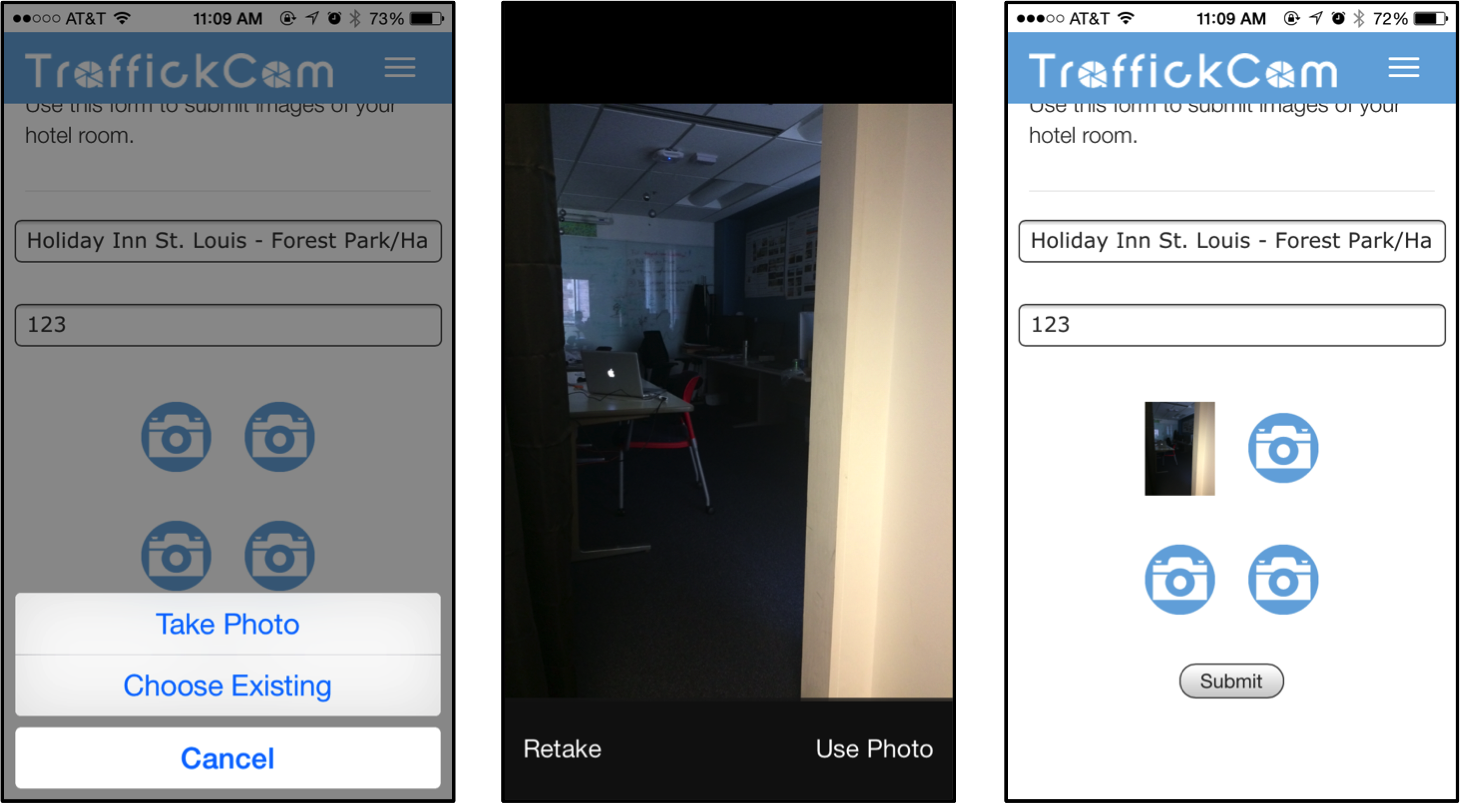
\includegraphics[width=\textwidth]{figs/chapter3/appScreenshots.png}
  \end{center}
  \caption[Smartphone app screenshots.]{Screenshots of the smartphone app, TraffickCam, that allows anyone to contribute to the database. The app is designed to require minimal user time and to protect the user's identity.}
  \label{fig:appScreenshots}
\end{figure*}

To supplement the images captured from existing datasets, we have created a smartphone crowd-sourcing application named TraffickCam, which allows travellers to upload their own photographs of a hotel room. This application is shown in Figure~\ref{fig:appScreenshots}. Users are asked to provide minimal information regarding the photo -- the name of the hotel they're staying in and their room number, along with images of the room.

The application, called TraffickCam, is available from the iOS and Android stores, in addition to being accessible via any modern browser at \url{http://traffickcam.org}.

Examples of images from both the Expedia dataset and the TraffickCam dataset, as well as representative images that law enforcement might upload to the TraffickCam system can be seen in Figure~\ref{fig:example_ims}.

\begin{figure*}[ht!]
  \begin{center}
  \begin{subfigure}[b]{\textwidth}
    \centering
    ~~~~~~~\includegraphics[width=.25\columnwidth]{figs/chapter3/expediaIms/1}
    \includegraphics[width=.25\columnwidth]{figs/chapter3/expediaIms/2}
    \includegraphics[width=.25\columnwidth]{figs/chapter3/expediaIms/3}
    \newline
    \includegraphics[width=.25\columnwidth]{figs/chapter3/expediaIms/4}
    \includegraphics[width=.25\columnwidth]{figs/chapter3/expediaIms/5}  
    \includegraphics[width=.25\columnwidth]{figs/chapter3/expediaIms/6} 
    \caption{Expedia Images}
  \end{subfigure}
  
  \begin{subfigure}[b]{\textwidth}
    \centering
    ~~~~~~~\includegraphics[width=.25\columnwidth]{figs/chapter3/traffickCamIms/1}
    \includegraphics[width=.25\columnwidth]{figs/chapter3/traffickCamIms/2}
    \includegraphics[width=.25\columnwidth]{figs/chapter3/traffickCamIms/3}
    \newline
    \includegraphics[width=.25\columnwidth]{figs/chapter3/traffickCamIms/4}
    \includegraphics[width=.25\columnwidth]{figs/chapter3/traffickCamIms/5}  
    \includegraphics[width=.25\columnwidth]{figs/chapter3/traffickCamIms/6}  
    \caption{TraffickCam Images}
  \end{subfigure}
  
  \begin{subfigure}[b]{\textwidth}
  \centering
    \includegraphics[height=120px]{figs/chapter3/backpage/3}
    ~~~~~~
    \includegraphics[height=120px]{figs/chapter3/backpage/1}
    ~~~~~~
    \includegraphics[height=120px]{figs/chapter3/backpage/2}
    \caption{Example Censored Query Images from Law Enforcement}
  \end{subfigure}
  
  \caption[Example images from TraffickCam and Expedia.]{The top set of images are from Expedia and the middle set of images taken by TraffickCam users at the same hotel. The bottom set of images are censored versions of the types of images that might be provided by law enforcement. These examples demonstrate the discrepancy in the types of photos provided by Expedia, by the TraffickCam app and by law enforcement.}
  \label{fig:example_ims}
  \end{center}
\end{figure*}

\section{Dataset Scope}
The present TraffickCam database includes 1,629,505 images from 150,289 unique hotels. Of these hotels, 131,244 hotels have only Expedia images, 15,242 have only TraffickCam images, and 10,742 hotels have both TraffickCam and Expedia images.

While the TraffickCam application purposefully collects no identifiable information about users to protect them from any legal action, we are able to estimate the number of users per hotel by the timestamp of the images uploaded -- the application asks users for a set of four images, so we assume images that are disjoint in time are from different users.

\section{Implementation Details}
We have implemented a RESTful API in Python Django, a web framework for rapid web development. Django handles the interaction between the server side code, web front end code, MySQL database and Apache web server. Test, stage and production Ubuntu environments are hosted through Amazon Web Services.

The iOS app, available through the Apple App Store, is simply a container that renders an HTML5+jQuery+AJAX web application hosted on~\url{https://traffickcam.org}, rather than a full native application. This allows for rapid development and easy exploration of different user experience choices (e.g., different motivational messages to display to users upon submission). The Android application is a native application available on the Google Play store.

\section{Application Statistics}
Since TraffickCam was released in December of 2015, there have been 68,700 installations on iOS devices and 28,500 installations on Android devices. These installations are primarily from users in the United States, where the search tool will first be deployed for law enforcement, but also include several thousand installations each from Europe and Asia. On average since the advertised release of the TraffickCam applications for iOS and Android in June of 2016, users have submitted just over 530 images a day.